\chapter{Team 3 Agent Design}\label{team_3_agent_design}

\section{The Agent}\label{sec:the_agent}
Team 3’s agents are based on the Theory of Reasoned Action (TRA). The agents are designed to have a shifting personality dependent on the three variables that this theory links to the behaviours of an agent. These three variables, together with a social network, define their personality as a whole, \cite{victor} and influence the actions they will take.\par
\begin{figure}[htb]
    \centering
    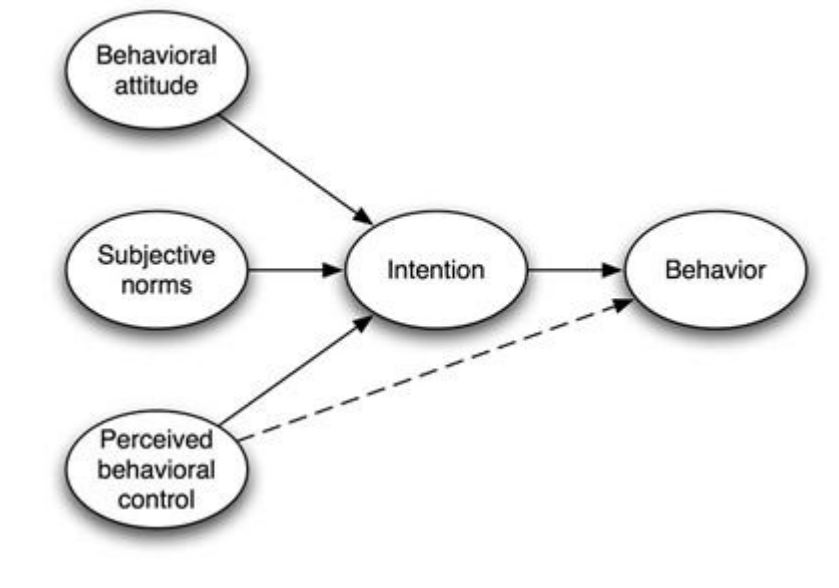
\includegraphics[width=0.5\linewidth]{005_team_3_agent_design/images/image1.jpg}
    \label{fig:TRA-diagram}
\end{figure}
The Theory of Reasoned Action was developed by Martin Fishbein in 1967. The TRA states that the behavioural intentions of individuals can be attributed to three interdependent factors: Perceived behaviour control, the subjective norm, and the attitude of the individual, as you can see in the figure above, \cite{norazalan}. Although it was recognised from the start, it must be noted that the TRA is unable to accurately and consistently predict non-volitional behaviours of the individual. Therefore, TRA can only be applied to those actions in which a reason can be found, actions that occur as a reaction to others and that the individual has control over, \cite{TRA}. This is applicable to our scenario, in which the agent must make a decision on how much food to eat after deliberating on their social network’s messages. \par
The application of TRA, in this case, is ideal given that reversing the methodology enables us to define an individual through the 3 core personality traits. The theory is a valid methodology to predict future behaviour by observing occurring actions and finding those components that caused them. Those components of behaviour can also be extrapolated to define an individual's behaviour and used to define it from the start. Therefore building the main characteristics of the personality of the individual, although lacking the uncontrollable or instinctive reactions. \par
Following the Theory of Reasoned Action, we have defined the agents’ emotion variables to be: 
\begin{enumerate}
    \item Stubbornness: it addresses perceived behaviour control, which is the influence that external agents have on the decisions that are to be taken. It is applied by the agent to ignore or read incoming messages and succumb or not to group pressure. 
    \item Morality: it addresses the subjective norm, which is one's idea of what is socially perceived to be right or wrong.
    \item Mood: it defines the attitude towards the action to take.
\end{enumerate}
These variables are modified as agents interact, which lead our agent to make different decisions during its time in the tower. All possible changes to these variables are done through ranges with the exact change each time being randomised, in other words inside a specified range any of the variables will change a different amount as a reaction for the same action. This course of action is based on the substantive uniqueness of each behaviour as defended by Martin Fishbein \cite{TRA}. This characteristic of randomness in the agents’ behaviour fulfilled the role of covering the fact that TRA does not take into account non-volitional behaviours, making the agent act as much as possible in a human-like behaviour. \par
The next step after identifying our agent strategy was to think about the scenario and how the problem should be solved. Our first approach used classical game theory, which states that under normal circumstances, an unbiased agent would always prioritise themselves and their needs over anything else. Hence, this dictates that each agent should not act in a moral way at all. In our scenario, this leads to agents taking selfish amounts of food, causing agents below to have less food and potentially die. However, we found research demonstrating how humans in a social environment tend to make decisions benefiting the collective, \cite{batson_batson_todd_brummett_shaw_aldeguer_1995}. This contradicted traditional game theory views and made this approach unreasonable when trying to recreate a human type behaviour, following the two most common explanations of why humans violate classic game theory: enlightened self-interest and group identity. 


\subsection{Action Process}
The Agent follows the following steps during their day: 
\begin{enumerate}
    \item The agent starts by updating their defining variables at the beginning of each day based on their HP. This acts as the agents checking in on themselves and changing their attitude(mood) and morality depending on their condition(HP).
    \item If the agent was just ‘born’ it will estimate an initial value for the average food consumed. 
    \item When the tower reshuffles the agents (which each agent knows by checking what floor they are on), the agent’s mood changes depending on the relative position of the new floor to the other floor. 
    \item The agent attempts to eat every day. The quantity depends on treaties, the messages they have received and whether other agents have requested them to leave or eat a certain amount of food or a calculation based on the agent’s current values. More information on this can be found in \Cref{sec:food_intake}. 
    \item Finally, the agent will attempt to communicate with other agents and create a social network via message sending and treaty proposition. More information on this is can be found in \Cref{sec:agent_communication}. 
  \end{enumerate}

\subsection{Agent Knowledge}
Agent 3 will be able to remember facts in order to make decisions. The information that is stored in their memory is:
\begin{enumerate}
    \item The floors the agent has been in before. This information will affect the agent’s mood after being reshuffled, as they would remember where they have been and know if the new floor is a good or bad one.  
    \item The last recorded HP value. Used to see changes in the agent's health.
    \item The agent’s friendship network. They are aware of the people they have met during their time in the tower. The agent’s friends are identified and are considered more or less close to the agent with an affection parameter that ranges from 0 to 1, 0  being complete dislike for the other agent.
    \item The amount of food last eaten.
    \item The amount of food last seen on the platform.
    \item A moving average of food consumed.
    \item The age of the agent.
    \item The treaty we have proposed until it is accepted or rejected.
    \item The estimation of the reshuffle.
    \item The HP our neighbour above last told us they had.
    \item The HP our neighbour below last told us they had.
\end{enumerate}

\subsection{Agent Generation}
The defining variables of our agents are randomised when they are generated in order to avoid preconditioned agents and mimic different personalities. All three variables are defined to be in the range 0 to 100. Morality and mood are randomly allocated to a value in the range, but stubbornness is limited to a number between 0 and 75. As explained in our agent parameters, stubbornness represents the effect of external influences on an agent. A stubbornness of 100 would mean this agent is completely unwilling to listen and would ignore all incoming messages, effectively making them an agent that disturbs the tower. In order for this to not be the case, we added the limitation to the value of stubbornness.\par
As Shao et al. have shown in “Beyond Moral Reasoning: A Review of Moral Identity Research and Its Implications for Business Ethics”, \cite{shao_aquino_freeman_2008}, one’s moral action is most heavily influenced by their moral personality, as opposed to their moral reasoning, which empirically seems to show only a minor influence on the moral behaviour of an agent, \cite{blasi_1983}. Hence, we used this variance and unpredictability to initialise our agents randomly on the moral scale. This insight also allowed us to witness a purely emergent strategy and nature as opposed to a pre-programmed inherent morality.\par
While the initial randomness allowed for interesting strategies to occur, we also wanted our agents to adapt their morality on the basis of their community and associations, as argued by Shao. Making it possible by having all actions an agent does affect its emotion variables. 

\section{Agent Communication}\label{sec:agent_communication}
Communication between agents is fundamental for the possibility of collaboration and self-organisation between agents. Crowd behaviour is considered to be generated by individuals, context-dependent and dynamic, as defended by the modern foundation of crowd behaviour, \cite{0d9bc1ee81234780b2bb6ecd02762d56}. In this project, communication between agents is based on two concepts, treaties and direct messages, which are equally exploited by our agent and combined with the conceptualization of friendship levels. 

\subsection{The Agent’s Social Network}
The agent forms relationships with others surrounding them as they communicate with each other. The agent remembers everyone they have met and assigns a level of friendship to them depending on their interactions. By doing this, the agent forms a social network that will affect their decisions, something that the Theory of Reasoned Action explores in the perceived behaviour control aspect of the theory. It is shown that all three main variables are linked together and for this reason, the agent will have a better or worse opinion of someone they have just met depending on their morality at that point. \par
Relationships are of high esteem for the agent as it follows the Aristotelian concept of friendship which defends friendship as “the finest way we exercise practical reasoning”. Quoting Aristotle: “Friendship seems to hold cities together, and lawgivers seem to care for it more than for justice … and when men are friends, they have no need for justice”. Friendship is considered the best form of human moral action by The Nicomachean Ethics, \cite{sokolowski}, and is fundamental in the decision-making process of the agent and its response to communication started by other agents. \par 
McCullough et al. investigate thoroughly the nature of prosocial action and gratitude’s place in transactions, \cite{doi:10.1111/j.1467-8721.2008.00590.x}. While this is difficult to realise fully in the code, we aimed to use the definitional guidelines set out, to relate our agent’s action and emotion to some of the more nuanced but socially beneficial emotions. Our friendship function allows us to assign a level of gratitude to our agent in response to the prosocial action of the other agents. In this way, we could more effectively alert the agent to the prosocial nature of another’s actions. By utilising the friendship function to, in turn, behave more prosocially to those who have done so to us, we embedded a system of gratitude in our agents’ actions. \par
We graduated our response by negotiating the selflessness of the action of the foreign agent. That is to say, in our game, the more severe the sacrifice on the behalf of the foreign actor, the more grateful we became. This is based on McCullough’s definition that one experiences gratitude when “they have benefited from someone’s costly, intentional, voluntary effort on their behalf”. \par 
Emotions allow us to respond to reality in a self-protective and self-enhancing way, \cite{ekman_1992}, it was this response we wanted our agent to have so that the emotions would govern their actions, by either leading them on a self-protective path, if circumstances such as selfish agents prevailed, or a self-enhancing manner, as cooperation would beget further cooperation through our system of gratitude.\par 
This is the basis of our friendship metric and implies our agent will react more positively to a friend and will increase the friendship of those with whom it has positive interactions.

\subsection{Message Sending}
Message sending is determined by a probabilistic decision, with each message having a 0.2 probability of being sent. The direction the messages are sent in is determined by the moral state of the agent. When the agent's morality is low, they will tend towards self-preservation and send messages upwards requesting information or help. On the other hand, when morality is high, the agent will look to create a stable society as stated by their willingness to look ahead and communicate with those below him to offer help and information, aiming to fortify their social network.\par 
The design of message passing has various noteworthy characteristics that act to aid the agent and occur if the conditions make it necessary: 
\begin{enumerate}
    \item The agent prioritises itself when its HP is critical, opting for treaties and messages that involve other agents leaving food in the platform and utilising this mechanic as a failsafe when in danger.
    \item The agents take into account the neighbours health when sending messages proposing how much food to leave on the platform. This makes the message more likely to be accepted. 
\end{enumerate}

\subsection{Message Reception}
When messages are involved, stubbornness is used to decide to ignore or read a message, with our reaction or answer also being dependent on the stubbornness of the agent. \par
The agent will follow the next process when a message is received:
\begin{enumerate}
    \item The agent will decide to ignore or read the message, with a probability of ignoring the message equal to the stubbornness level.
    \item If the agent decides to read the message it is analysed and matched with the type of response or responses acceptable for the message. 
    \item The agent will note the agent that sent the message and consider the friendship level it shares with the sender. Friendship together with the morality level and the content of the message itself will decide the exact content of the response.
    \item The content of the message and its sender will affect the agents’ emotional variables and the friendship level with the sender. This change affects the future reaction to communication done by other agents and the decisions taken by the agent from that point onwards. 
\end{enumerate}
To ensure a minimum level of communication all messages read will be answered by the agent. 

\subsection{Reaction to Received Messages}
The changes are dependent on four criteria to determine initial agent characteristic manipulation. These four variables are the variables present upon the receipt of the message and somewhat representative of the type 1 brain system discussed in \cite{kahneman_tversky_2000}, \cite{frankish_2010}. \par
The initial emotional response is based on the variables of the immediate past, the hp moving average on the last five ticks, opposed to the overall hp average, or welfare average. This is to represent the subconscious layer of emotional response, as seen in, \cite{kamble_2021}, whereby our response to the situation is more irrational and illogical than the conscious mind perceives. \par
Summing the net total of all the initial responses to zero, allows us to explore the oscillatory nature of emotion while avoiding the possible pitfall of any dominant emotions. \par
\begin{table}[htb]
    \centering
    \begin{tabular}{@{}lllll@{}}
    \toprule
    HP dec last tick [nonfriend]    & Stubbornness      & Morality         & Mood             & Friendship     \\ \midrule
    ask Food Taken                  & 0                 & -0.5             & -0.5             & 0              \\
    ask HP                          & 0                 & -0.5             & -0.5             & 0              \\
    ask Intended Food Intake        & 0                 & 0                & 0                & 0              \\
    Request Take Food               & 1                 & -0.5             & -1               & -1             \\
    Request Leave Food              & 1                 & -0.5             & -1               & 0              \\ \bottomrule
    \end{tabular}
\end{table}
\begin{table}[htb]
    \centering
    \begin{tabular}{@{}lllll@{}}
    \toprule
    HP inc last tick [nonfriend]    & Stubbornness      & Morality         & Mood             & Friendship     \\ \midrule
    ask Food Taken                  & 0                 & 0                & 0                & -1             \\
    ask HP                          & -1                & 1                & 1.5              & 1              \\
    ask Intended Food Intake        & 0                 & 0                & 0                & 0              \\
    Request Take Food               & 0                 & 0                & 0                & 0              \\
    Request Leave Food              & -1                & 1                & 1.5              & 1              \\ \bottomrule
    \end{tabular}
\end{table}
\begin{table}[htb]
    \centering
    \begin{tabular}{@{}lllll@{}}
    \toprule
    Sum total                       & Stubbornness      & Morality         & Mood             & Friendship     \\ \midrule
    Request Leave Food              & 0                 & 0                & 0                & 0              \\ \bottomrule
    \end{tabular}
\end{table}
This zero-sum agent is how our agent is currently set, it represents the neutral agent. One who possesses no inherent emotional bias. This was done by balancing the positive and negative reactions to a friend, and those to a non-friend separately. We noticed the need for this when our agent would initially get stuck at the +ve and -ve limits of certain emotions. As future work, it would be exciting to see the emergent strategies which we hope to observe as we introduce biases. For instance, an agent whose net sum of all interactions leaves them with a stubbornness increase, coupled with an inherently moral agent, may create strategies yet thought of. 

\subsection{Proposing a Treaty}
When the agent HP is critical, they will ask for help by either asking for the person upstairs to leave at least the amount of food necessary to survive or, if it doesn’t have any active treaties, a treaty that states: if HP is higher than 20 leave 95\% of the food in the platform for 3 days. At this time the agent's self-preservation instinct takes precedence and their objective becomes to eat enough food to get out of the critical state before the agent dies.
When the agent is not in critical condition, it will be able to propose other treaties depending on their morality. The first treaty is detrimental for the tower and the other two are ‘fair’ treaties for the tower. \par
\begin{enumerate}
    \item If the agent is very immoral, it will send a treaty that is detrimental for anyone above them. It is expected for this treaty to be rejected by any sensible agents and is done as a way of mimicking frustration or the desire to hurt others when morality is low.
    \item If HP is below 60 leave at least 60\% of the food on the platform for 5 days. This treaty tries to encourage immoral agents in higher positions to share food. 
    \item If HP is below 10 leave at least 95\% of the food on the platform for 10 days. This treaty is aimed at moral agents that would be willing to start eating less until they are close to death.
\end{enumerate}
Both of the last treaties are proposed randomly by the agent, without a specific proclivity for any of the two. The randomness of the treaty selection is done to increase the volitional behaviour of the agent. Characteristics that the agent inherently lacks if its personality is solely based on the TRA.

\subsection{Handling a Proposed Treaty}
Following our strategy, agents that are in a bad mood will not accept treaties that they need to honour when they are in very low health, since they have low confidence in the capabilities of other agents. However, when in a good mood agents will accept treaties that must be honoured even at low health. Morality is an indicator of the agent’s desire to perform actions that will benefit others, as opposed to just benefiting the agent itself. Therefore, very moral agents will accept treaties that involve them consuming just enough food to survive, but not too little food that they die or too much that they are too greedy. Similarly, very immoral agents will only accept treaties where they consume more than enough food since they disregard the food needs of the other agents. The table below displays the mood and morality values that agents must satisfy to accept treaties with any given condition depending on the agent’s health, and the food the agent would have to leave according to the request of the treaty. \par
\begin{table}[htb]
    \centering
    \resizebox{\textwidth}{!}{\begin{tabular}{|l|l|l|l|l|l|l|l|}
    \hline
        mood (m)/morality (M)   & ~                                     & 0 $<$ morality $<$ 40     & 20 $<$ morality $<$ 60    & 40 $<$ morality $<$ 80    & 60 $<$ morality $<$ 100   & morality $>$ 80       & morality $>$ 100      \\ \hline
        ~                       & AgentPosition $\backslash$ FoodTaken  & VeryLarge (1)             & Large (2)                 & Moderate (3)              & Little (4)                & SurvivalAmount (5)    & TooLittle (6)         \\ \hline
        mood $>$ 0              & Strong (1)                            & m$>$0, 0$<$M$<$40         & m$>$0, 20$<$M$<$60        & m$>$0, 40$<$M$<$80        & m$>$0, 60$<$M$<$100       & m$>$0, 80$<$M         & N/A since 100$<$M     \\ \hline
        mood $>$ 20             & Healthy (2)                           & m$>$20, 0$<$M$<$40        & m$>$20, 20$<$M$<$60       & m$>$20, 40$<$M$<$80       & m$>$20, 60$<$M$<$100      & m$>$20, 80$<$M        & N/A since 100$<$M     \\ \hline
        mood $>$ 40             & Average (3)                           & m$>$40, 0$<$M$<$40        & m$>$40, 20$<$M$<$60       & m$>$40, 40$<$M$<$80       & m$>$40, 60$<$M$<$100      & m$>$40, 80$<$M        & N/A since 100$<$M     \\ \hline
        mood $>$ 60             & Weak (4)                              & m$>$60, 0$<$M$<$40        & m$>$60, 20$<$M$<$60       & m$>$60, 40$<$M$<$80       & m$>$60, 60$<$M$<$100      & m$>$60, 80$<$M        & N/A since 100$<$M     \\ \hline
        mood $>$ 80             & SurvivalLevel (5)                     & m$>$80, 0$<$M$<$40        & m$>$80, 20$<$M$<$60       & m$>$80, 40$<$M$<$80       & m$>$80, 60$<$M$<$100      & m$>$80, 80$<$M        & N/A since 100$<$M     \\ \hline
    \end{tabular}}
\end{table}
Treaties also have a specified duration and signature count, which are visible to any agent that wishes to sign the treaty. These are likely to affect an agent’s decision to accept a treaty and have been taken into account. If a treaty lasts longer than twice the reshuffle period, an agent deems it too far into the future to be able to predict what will happen and plans to reject the treaty. However, if a treaty has more than five signatures, we deem it to be a popular treaty. If the agent plans to reject the treaty as a result of any previous logic, the influence of peer pressure will cause the agent to reconsider accepting the treaty. Peer pressure is based on the concept of crowd suggestibility coined by Park, R. E.  in 1904 in his “Masse und Publikum”, \cite{Solr-413687}. The stubbornness of an agent is used as the likelihood to give in to peer pressure, so more stubborn agents are less likely to reconsider their response, and more likely to stick with their original decision. \par

\section{Food Intake}\label{sec:food_intake}
For an agent to choose what to eat on a given day, they first take into account treaties to which they have agreed. These treaties take the highest priority when deciding how much food to take from the platform. Therefore, when the agent in question has accepted a treaty the choice becomes dependent on the treaty conditions. \par 
For each treaty that has been accepted, the agent follows the following logic: 
\begin{enumerate}
    \item They start by checking whether the condition stated within the specific treaty is satisfied, in which case the agreed-upon amount of food to leave on the platform is calculated. 
    \item In the case where the treaty request is not to leave food on the platform but to inform the sender of the treaty of our agent's HP, a message containing our current HP is sent to the sender agent. 
\end{enumerate}
After all the treaty conditions have been dealt with the agent calculates how much food to eat itself. The calculation depends on the morality of the agent, how much food it has decided to leave on the platform and how much food it has decided to eat. It must be noted that during other processes external to the final decision of how much to eat the agent might have decided how much it would like to eat, i.e a non-binding decision. \par
Depending on the agents’ decision regarding how much food to eat and leave it will arrive at 4 possible scenarios: 
\begin{enumerate}
    \item If it has decided how much food to eat and leave and both conditions can be met the agent will eat. If meeting both conditions is impossible, there is not enough food on the platform, a decision that fulfils the value of how much food to leave will be taken, with the value of how much the agent eats ranging from all that it can to just what it needs to survive. 
    \item If the agent knows how much it wants to eat but not how much to leave it will attempt to eat the amount it has decided it wants.
    \item If the agent has not decided how much to eat but knows how much to leave it will eat depending on its health condition. If its health is critical or about to die it will eat whatever it needs to survive. If its health is not of concern it will eat as much as it can while leaving the amount it has decided to leave. Morality is used to scale how much food to eat.
    \item If it is unaware of how much to leave or eat its decision will depend on its health level. If its health is critical or about to die it will eat whatever it needs to survive. If its health is not of concern, eat an amount of food scaled by its morality.
\end{enumerate}